\section{Grundlagen}[ht] \label{sec:Grundlagen}
In diesem Abschnitt werden die grundlegenden Konzepte und Begriffe erläutert, die für das Verständnis dieser Arbeit notwendig sind. Zunächst werden Software-Qualitätsmetriken vorgestellt, da sie die Basisdaten für alle in dieser Arbeit genutzten Visualisierungen liefern. Anschließend wird das Thema Software-Visualisierung behandelt, wobei insbesondere auf die dreidimensionale Software-Visualisierung mit Hilfe von Treemaps eingegangen wird.

\subsection{Software-Qualitätsmetriken} \label{sec:SoftwareQualitaetsmetriken}

Software-Qualitätsmetriken sind zentrale Werkzeuge zur Messung und Bewertung der Qualität von Software. Sie ermöglichen es, verschiedene Eigenschaften der Software objektiv anhand von Kennzahlen zu analysieren. Eine \textit{Softwaremetrik} ist dabei meist als mathematische Funktion zu verstehen, die eine spezifische Eigenschaft einer Software in einen Zahlenwert abbildet:

\begin{quote}
    Eine Softwaremetrik, oder kurz Metrik, ist eine (meist mathematische) Funktion, die eine Eigenschaft von Software in einen Zahlenwert, auch Maßzahl genannt, abbildet. Hierdurch werden formale Vergleichs- und Bewertungsmöglichkeiten geschaffen.\cite{wikipedia_softwaremetrik}
\end{quote}

Auch in anderen Definitionen wird die grundsätzliche Funktion von Metriken hervorgehoben:

\begin{quote}
    Softwaremetrik ist ein quantitatives Maß, das verwendet wird, um die Eigenschaften eines Softwareproduktes oder des Softwareentwicklungsprozesses zu bewerten.\cite{softwaremetriken_2019}
\end{quote}

\begin{quote}
    Eine Softwarequalitätsmetrik ist eine Funktion, die eine Software-Einheit in einen Zahlenwert abbildet, welcher als Erfüllungsgrad einer Qualitätseigenschaft der Software-Einheit interpretierbar ist.\cite{def_qual_metric}
\end{quote}

Allen Definitionen ist gemeinsam, dass eine Metrik stets nur einen bestimmten Aspekt der Software abbildet. Genau darin liegt eine der wichtigsten Erkenntnisse und gleichzeitig eine zentrale Kritik: Einzelne Metriken geben ausschließlich Auskunft über spezifische Eigenschaften und erlauben keine umfassende Bewertung der gesamten Softwarequalität.

Zusammenfassend kann festgestellt werden, dass Software-Qualitätsmetriken als quantitative Indikatoren zur Kontrolle und Verbesserung der Software dienen. Sie sind jedoch stets darauf beschränkt, nur bestimmte Aspekte zu messen. Die Aussagekraft jeder einzelnen Metrik ist daher begrenzt:

\begin{quote}
    Eine Metrik alleine kann nie eine vollständige Aussage über die Qualität der Software treffen. Metriken sollten immer in Kombination bewertet werden. Die Güte und Reife von Software kann nur in Kombination mit statischer Code Analyse, Code Reviews und funktionalen Tests final beurteilt werden.\cite{schmitz_2019}
\end{quote}

Es existiert also keine universelle Metrik, die vollumfänglich Auskunft über die Qualität einer Software geben kann. Dies allein schon, da der Begriff \textit{gute Software} situationsabhängig definiert werden muss. Selbst wenn fehlerfreie Ausführung als Ziel gilt, ist unklar, wie diese Eigenschaft in eine einzelne Metrik gefasst werden könnte.

Um ein möglichst vollständiges Qualitätsbild zu erhalten, ist es daher essenziell, verschiedene Metriken miteinander zu kombinieren. Die parallele Interpretation mehrerer Indikatoren erhöht die Aussagekraft und reduziert das Risiko von Fehleinschätzungen.

\smallskip


Die Aussagekraft von Softwaremetriken hängt maßgeblich davon ab, dass die Ziele der Software klar definiert sind \cite{hall1994implementing}. Metriken müssen stets so gewählt werden, dass sie die Qualität einer Software bezüglich dieser Ziele abbilden. Beispielsweise ist eine Komplexitätsmetrik irrelevant, wenn primär die Ausführungsgeschwindigkeit optimiert werden soll. Auch kann die Erhebung und Auswertung von Metriken selbst mit Aufwand verbunden sein.

Ein weiterer Kritikpunkt ist, dass viele Metriken nicht ausreichend wissenschaftlich fundiert sind und der tatsächliche Nutzen nicht immer klar belegt werden kann \cite{voas_kuhn_2017}. Die Orientierung an Metriken sollte daher immer kritisch erfolgen und nicht zum Selbstzweck werden.

Zudem besteht die Gefahr, dass bei unpassend gewählten Metriken lediglich diese Werte optimiert werden, ohne dass sich dadurch die Gesamtqualität der Software verbessert. Entwickler könnten dazu verleitet werden, ihr Handeln auf das Erreichen guter Metrikwerte anstatt auf das eigentliche Ziel der Software auszurichten \cite{worst_gitclear_2025}.

Nicht zuletzt sind Metriken kontextabhängig. Sie liefern Indizien, können aber Prozesse wie Code Reviews oder Tests keinesfalls ersetzen. Die Interpretation muss mit Blick auf den jeweiligen Kontext erfolgen. Bekannte Beispiele wie Lines-of-Code oder Anzahl von Commits werden oft falsch als Qualitätsindikatoren genutzt, obwohl sie weder die Komplexität noch die tatsächliche Arbeitsleistung adäquat abbilden \cite{worst_gitclear_2025}.

Einfache Metriken können zudem keine komplexen Qualitätsprobleme identifizieren \cite{voas_kuhn_2017} und sind häufig stark abhängig von Programmiersprache und individuellem Programmierstil.

\smallskip


Die Norm ISO/IEC 25010 \cite{iso25010_2024} beschreibt einen Rahmen, in dem die Qualität von Software anhand von acht Qualitätsmerkmalen, wie z.B. funktionaler Eignung, Zuverlässigkeit oder Benutzerfreundlichkeit, strukturiert wird. Diese Merkmale beziehen sich auf die Sicht von außen, also wie der Benutzer die Software erlebt:

\begin{quote}
    Qualität wird als Abwesenheit von Fehlern im Systemverhalten verstanden, die Software verhält sich demnach so, wie der Benutzer es erwartet.\cite[1]{Witte2018}
\end{quote}

Für die Ursachen bestimmter Qualitätsprobleme reicht die Betrachtung aus Nutzersicht allerdings oft nicht aus. Seit den 1970er Jahren entstand daher ein Fokus auf die Messung der \textit{internen Qualität} beziehungsweise der \textit{Code-Qualität}, etwa mittels Metriken wie der McCabe-Komplexität \cite{ludewig}. Diese ist insbesondere für Entwickler sowie Auftraggeber relevant und unterstützt die Sicherstellung von Wartbarkeit und Erweiterbarkeit der Software. Im Rahmen dieser Arbeit wird, soweit von Metriken die Rede ist, explizit auf Code-Qualitätsmetriken Bezug genommen.

\smallskip


Software-Qualitätsmetriken beziehen sich in der Regel auf spezifische Softwareeinheiten, beispielsweise Dateien, Module oder Klassen. Diese Einheiten sind meistens hierarchisch, etwa entlang von Datei- und Ordnerstrukturen, organisiert. Die Messwerte werden häufig auf der Ebene einzelner Dateien gesammelt und dann auf höhere Ebenen, zum Beispiel Ordner oder Module, aggregiert, sodass eine baumartige Hierarchie entsteht.

Die im Folgenden vorgestellten Ansätze zur Visualisierung hierarchischer Metrik-Daten sind nicht zwingend spezifisch für Softwaremetriken, sondern lassen sich auch auf andere Anwendungsfälle übertragen. Dennoch weist die Struktur von Software-Einheiten und deren Metrik-Daten gewisse Eigenheiten auf, was Einfluss auf die Gestaltung der Visualisierungen haben kann (siehe Abschnitt \ref{INPUT DATEN ANALYSE}).

\subsection{Software-Visualisierung} 
\label{sec:SoftwareVisualisierung} 

Die Darstellung von Softwarestrukturen zählt zu den entscheidenden Schritten, um komplexe Softwaresysteme für Menschen verständlich zu machen. Während numerische Metriken oder tabellarische Darstellungen für Fachleute in der Softwareentwicklung oft ausreichend sind, können diese Darstellungsformen für Personen ohne technischen Hintergrund abstrakt und schwer zugänglich bleiben. Es besteht daher das Ziel, Softwarequalität auch für nicht-technische Stakeholder intuitiv und erlebbar zu machen.

HIER NOCH QUELLEN UND BISSCHEN WAS ZU DER HISTORIE UND WARUM WIESO PIPAPO

\subsection{3D-Software-Visualisierung} \label{sec:3DSoftwareVisualisierung}

Traditionell werden Softwaremetriken in numerischer oder zweidimensionaler Form präsentiert. Diese Formen liefern zwar einen guten Überblick, vermitteln jedoch wenig \textit{Greifbarkeit} des Softwaresystems. 3D-Visualisierungen bieten dagegen das Potenzial, immersive und erfahrbare Eindrücke zu schaffen, sodass Nutzer \textit{in die Software eintauchen} können:
\begin{quote}
Despite the proven usefulness of 2D visualizations, they do not allow the viewer to be immersed in a visualization, and the feeling is that we are looking at things from 'outside'. 3D visualizations on the other hand provide the potential to create such an immersive experience \cite[1]{codeCity1}
\end{quote}

Die Idee, Softwarestrukturen dreidimensional darzustellen, ist nicht neu. Bereits 1995 stellte Steven P. Reiss einen ersten Ansatz zur 3D-Visualisierung von Software vor \cite{first_3D_vis}. Ursprünglich zielten diese Ansätze darauf ab, Entwicklern einen schnellen Überblick über Struktur und Aufbau umfangreicher Systeme, insbesondere beim Einarbeiten in unbekannte Software, zu verschaffen \cite{visSoftwareVR}. Die frühen Methoden fokussierten dabei meist die Darstellung von Architektur und Verbindungen, weniger jedoch die Visualisierung von Softwarequalitätsmetriken (siehe Abbildung \ref{fig:3DVis}).

\begin{figure}[h]
    \centering
    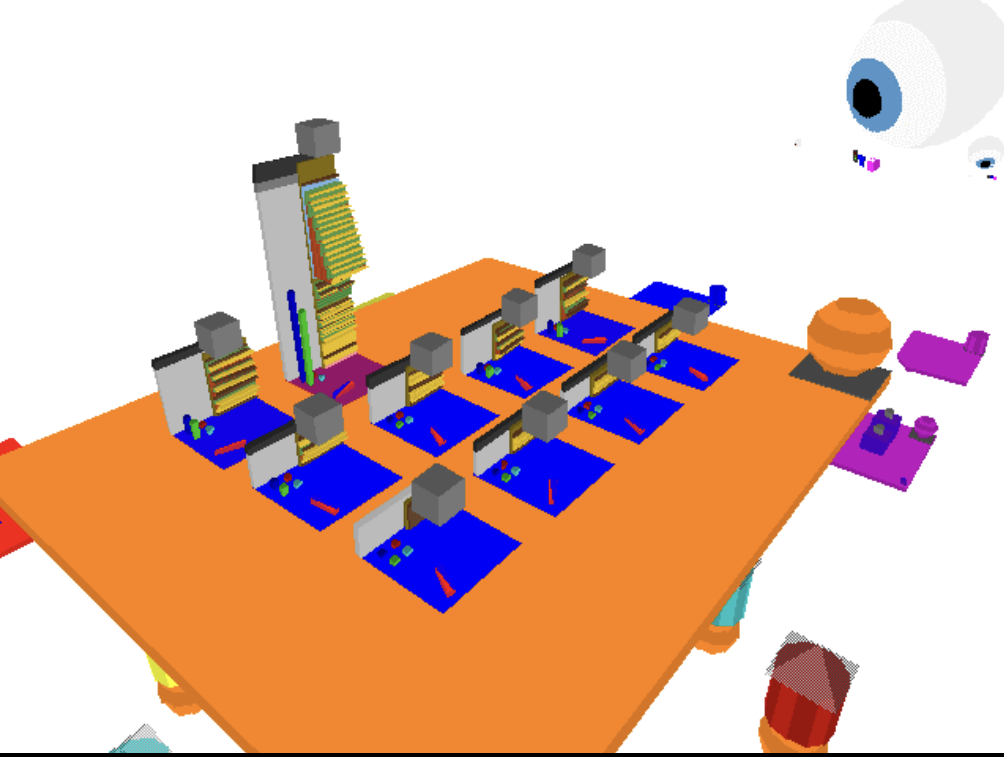
\includegraphics[width=0.5\textwidth]{images/visVRExample.png}
    \caption{Beispiel für eine 3D-Visualisierung von Young und Munro \cite[6]{visSoftwareVR}}
    \label{fig:3DVis}
\end{figure}

Für die Visualisierung von Softwarequalitätsmetriken lassen sich aus der Literatur Kriterien für eine gelungene 3D-Darstellung ableiten \cite{visSoftwareVR}:
\begin{itemize}
    \item \textbf{Darstellung der Struktur:} Die Visualisierung soll Architektur und Aufbau der Software möglichst anschaulich und nachvollziehbar zeigen. Wichtige Aspekte dabei sind:
    \begin{itemize}
        \item \emph{Informationsgehalt:} Die Darstellung soll möglichst viele relevante Informationen kompakt vermitteln.
        \item \emph{Visuelle Komplexität:} Trotz hoher Informationsdichte soll die Visualisierung übersichtlich und nicht überfordernd wirken. Dies ist als Gegenspieler zum Informationsgehalt zu verstehen.
        \item \emph{Skalierbarkeit:} Auch große Softwaresysteme müssen klar und verständlich dargestellt werden können. Die Autoren von \textit{Visualising Software in virtual reality} \cite{visSoftwareVR} sagen sogar, dass Mechanismen notwendig wären, um Komplexität und Informationsgehalt bei zunehmender Größe manuelll zu steuern und je nach Software-System anpassen zu können.
        \item \emph{Stabilität gegenüber Änderungen:} Die Visualisierung soll bei Software-Änderungen konsistent bleiben, um Vergleichbarkeit über Versionen hinweg zu gewährleisten.
        \item \emph{Visuelle Metaphern:} Der Einsatz eingängiger Metaphern erleichtert das Verständnis komplexer Softwarestrukturen.
    \end{itemize}
    \item \textbf{Abstraktion:} Unwesentliche Details sollten ausgeblendet werden, um ein verständliches, abstrahiertes Modell zu erzeugen.
    \item \textbf{Navigation:} Die Orientierung innerhalb der Visualisierung muss auch bei sehr großen Systemen einfach und intuitiv möglich sein.
    \item \textbf{Korrelation mit dem Code:} Es sollte eine klare Zuordnung zwischen Visualisierungselementen und Quellcodebestandteilen existieren.
    \item \textbf{Automatisierung:} Die Generierung der Visualisierung sollte vollständig automatisierbar sein, sodass keine manuelle Nachbearbeitung notwendig ist.
\end{itemize}

\subsubsection{CodeCity: Grundstein für 3D-Visualisierung}
\label{sec:CodeCity}

Eine prägende Arbeit für die 3D-Visualisierung von Softwarestrukturen und -metriken ist das Konzept \textit{CodeCity} von Richard Wettel und Michele Lanza \cite{codeCity1}. Sie stellten erstmals einen Ansatz vor, der Software-Struktur auf Modulebene nutzt, um den Grundriss für eine 3D-Visualisierung zu schaffen. Dabei werden Softwareeinheiten als als Quader dargestellt. Wie von Young und Munro \cite{visSoftwareVR} gefordert, nutzen sie eine gute visuelle Metapher, um die Software darzustellen: die Stadtmetapher. Sie ist zentrales Gestaltungsmittel von CodeCity: Klassen erscheinen als Gebäude, Pakete als Stadtbezirke. Den Objekten werden verschiedene Attribute (Dimensionen, Positionen, Farben, Farbsättigung, Transparenz) zugeordnet, was eine intuitive und greifbare Darstellung ermöglicht (siehe Abbildung \ref{fig:codeCity}).

\begin{figure}
    \centering
    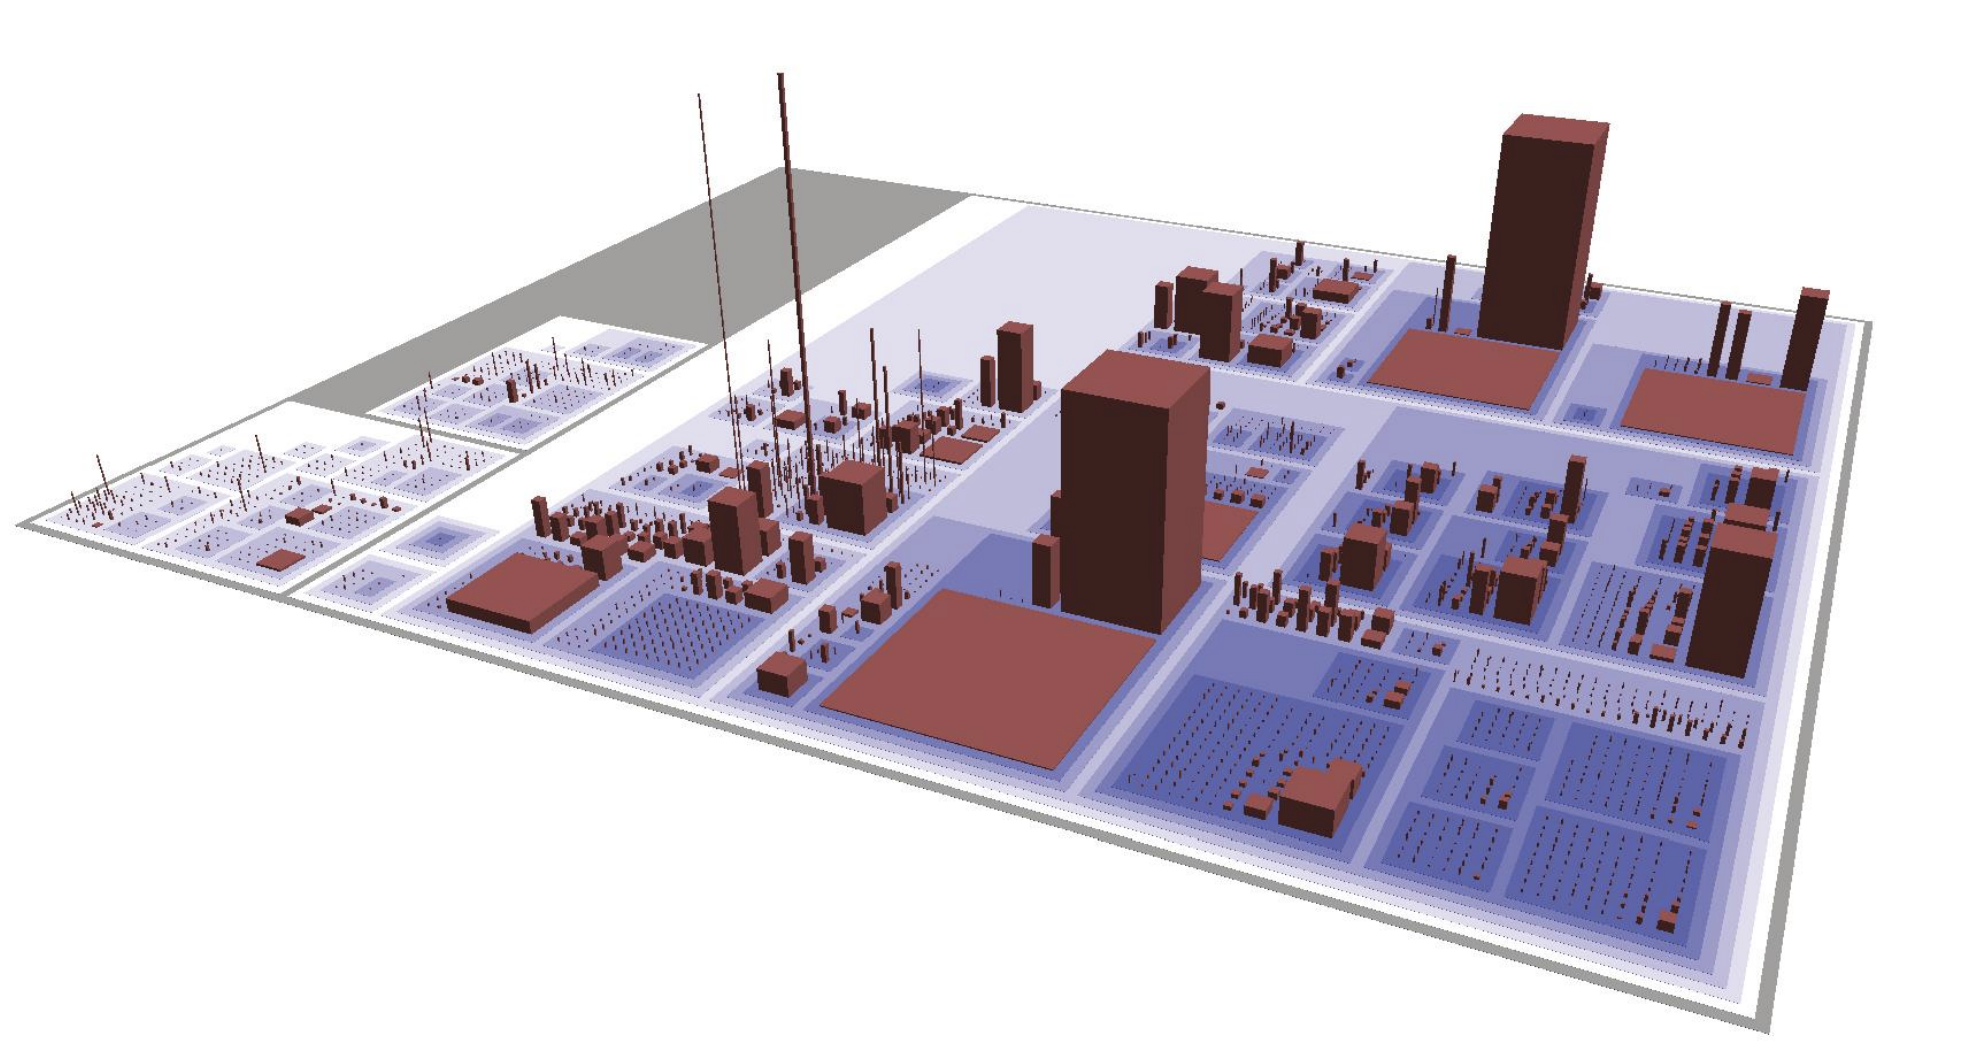
\includegraphics[width=0.5\textwidth]{images/codeCityExample.png}
    \caption{Beispiel für eine originale CodeCity-Visualisierung~\cite[2]{codeCity1}}
    \label{fig:codeCity}
\end{figure}

Während frühere Arbeiten, wie die von Marcus et al. \cite{3dsoftwareMarcus}, auf sehr feingranulare Codebestandteile, wie Attribute und Methoden, fokussierten, bietet CodeCity eine abstrahierende Sicht auf Klassen, Pakete und deren Struktur und ist dadurch vorallem für nicht-technische Stakeholder verständlicher und leichter zu überblicken.

Der Grundriss (folgend auch Layout) der Städte beruht auf einer Variante der Treemap-Algorithmen (erklärt im folgenden Abschnitt \ref{sec:Treemap}). Es ist zu erkennen, dass größere Gebäude im unteren linken Bereich, kleinere weiter oben rechts angeordnet sind. Gebäude (Module) und Viertel (Pakete) sind immer quadratisch, dadurch bleibt viel ungenutze \textit{leere} Fläche. 

Das Originalverfahren des CodeCity-Algorithmus ist nicht öffentlich verfügbar. In dieser Arbeit wird daher für vergleichende Analysen eine eigene Implementierung verwendet, so dass Abweichungen zur Originalvisualisierung möglich sind (außer wenn anders gekennzeichnet).

\subsection{Treemap-Layouts} \label{sec:Treemap}

Hierarchische Daten werden häufig als Bäume dargestellt, jedoch zeigen sich klassische Darstellungen wie Baumdiagramme oder Venn-Diagramme insbesondere bei großen Datenmengen als ineffizient hinsichtlich der Flächennutzung und generell unübersichtlich \cite{johnson1991tree}. Besonders für große, strukturreiche und mengenorientierte Daten stoßen traditionelle Visualisierungsmethoden an ihre Grenzen, da sie weder Informationen noch Hierarchien kompakt und intuitiv vermitteln können.

Um diese Herausforderungen zu adressieren, entwickelten Shneiderman und Johnson 1991 das Konzept der \textit{Treemap} zur effizienten Darstellung hierarchischer Strukturen \cite{johnson1991tree}.
Das zentrale Prinzip von Treemaps besteht darin, jedem Knoten eines gewichteten Baums ein Rechteck zuzuweisen, dessen Fläche proportional zu dem Gewicht (beispielsweise Datenmenge, Marktwert, o. ä.) ist.
Die Rechtecke aller Blätter füllen die Fläche des Wurzelrechtecks vollständig aus, sodass die Gesamtfläche der Kindknoten exakt der Fläche ihres Elternrechtecks entspricht. Mathematisch liegt der Visualisierung also ein gewichteter Baum zugrunde, wobei insbesondere die Blattknoten jeweils einen numerischen Wert besitzen.

Shneiderman und Johnson identifizieren für gelungene Treemaps folgende Schlüsselziele:
\begin{itemize}
    \item \textbf{Effiziente Platznutzung:} Maximale Informationsdichte auf minimalem Raum.
    \item \textbf{Verständlichkeit:} Einfache Erfassbarkeit der dargestellten Hierarchie und Werte mit geringem kognitiven Aufwand. Die Struktur soll möglichst schnell erkennbar sein.
    \item \textbf{Ästhetik:} Ansprechende und übersichtliche Anordnung der Rechtecke.
\end{itemize}

Frühere Ansätze wie Listen, klassische Baumdiagramme (Abbildung \ref{fig:baumdiagramm}) oder Venn-Diagramme (Abbildung \ref{fig:venndiagram}) konnten diese Anforderungen nicht erfüllen. Sie leiden unter Problemen wie ineffizienter Flächenausnutzung und fehlender Möglichkeit, zusätzlich zu den Beziehungen auch quantitativ-metrische Informationen anschaulich zu vermitteln. So kann zum Beispiel in klassischen Baumdiagrammen bei großen Datenmengen mehr als die Hälfte des dargestellten Bereichs aus leerem, informationslosem Raum bestehen \cite[3]{johnson1991tree}. Venn-Diagramme sind insbesondere aus Platzgründen für größere Strukturen ungeeignet: \enquote{The space required between regions would certainly preclude this Venn diagram representation from serious consideration for larger structures.}\cite[5]{johnson1991tree}

\begin{figure}[ht]
    \centering
    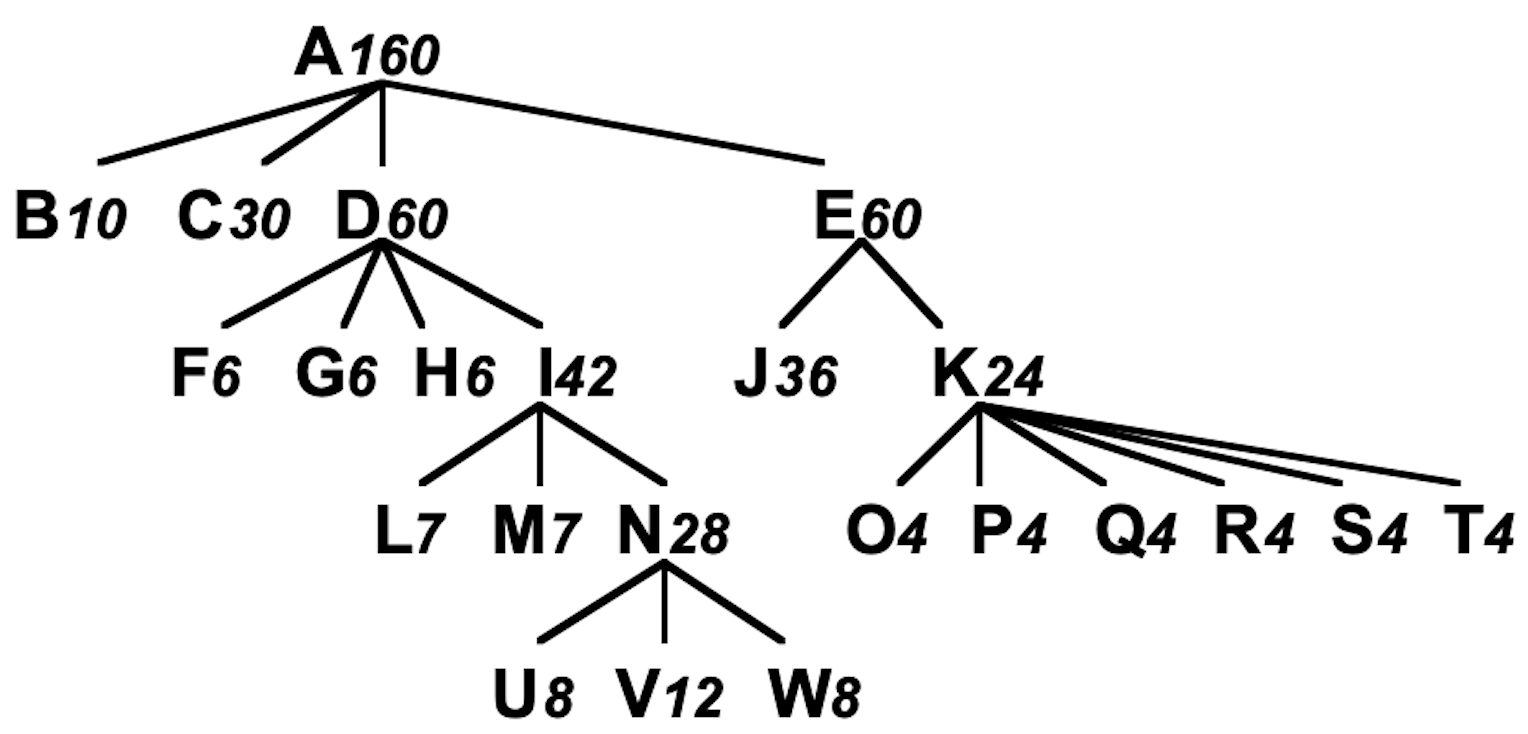
\includegraphics[width=0.5\textwidth]{images/treediagram.png}
    \caption{Beispiel für ein Baumdiagramm}
    \label{fig:baumdiagramm}
\end{figure}

\begin{figure}[ht]
    \centering
    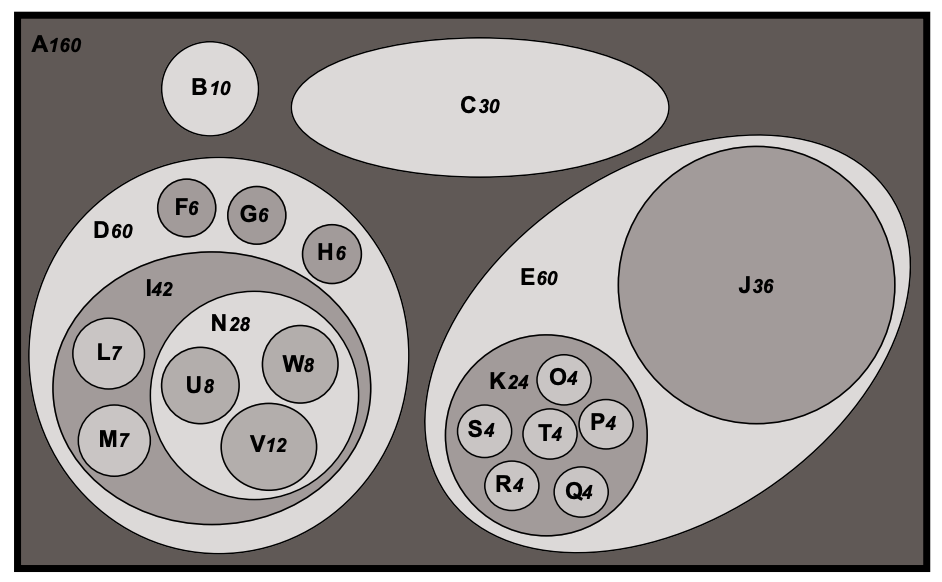
\includegraphics[width=0.5\textwidth]{images/verdiagram.png}
    \caption{Beispiel für ein Venn-Diagramm}
    \label{fig:venndiagram}
\end{figure}

Um die genannten Schwierigkeiten zu lösen, formulieren Shneiderman und Johnson vier grundlegende Eigenschaften für Treemap-Layouts:
\begin{itemize}
    \item Ist Knoten 1 ein Vorfahre von Knoten 2, so ist der Bereich von Knoten 2 vollständig innerhalb des Bereichs von Knoten 1 enthalten.
    \item Die Bereiche von Knoten schneiden sich, wenn einer ein Vorfahre des anderen ist.
    \item Jeder Knoten erhält eine Fläche, die streng proportional zu seinem Gewicht ist.
    \item Das Gewicht eines Knotens ist (mindestens) so groß wie die Summe der Gewichte seiner Kinder.
\end{itemize}

Sie präsentieren einen einfachen, rekursiven Algorithmus, der diese Bedingungen erfüllt: Der verfügbare Raum wird abwechselnd vertikal und horizontal entsprechend den Gewichten der Kindknoten aufgeteilt. Die Berechnung erfolgt von der Wurzel bis zu den Blättern und ist mit einer Laufzeit von $O(n)$ effizient. Ein Beispiel für eine Treemap, die mit diesem Algorithmus erstellt wurde, ist in Abbildung \ref{fig:nestedTreemap} zu sehen.

\begin{figure}[ht]
    \centering
    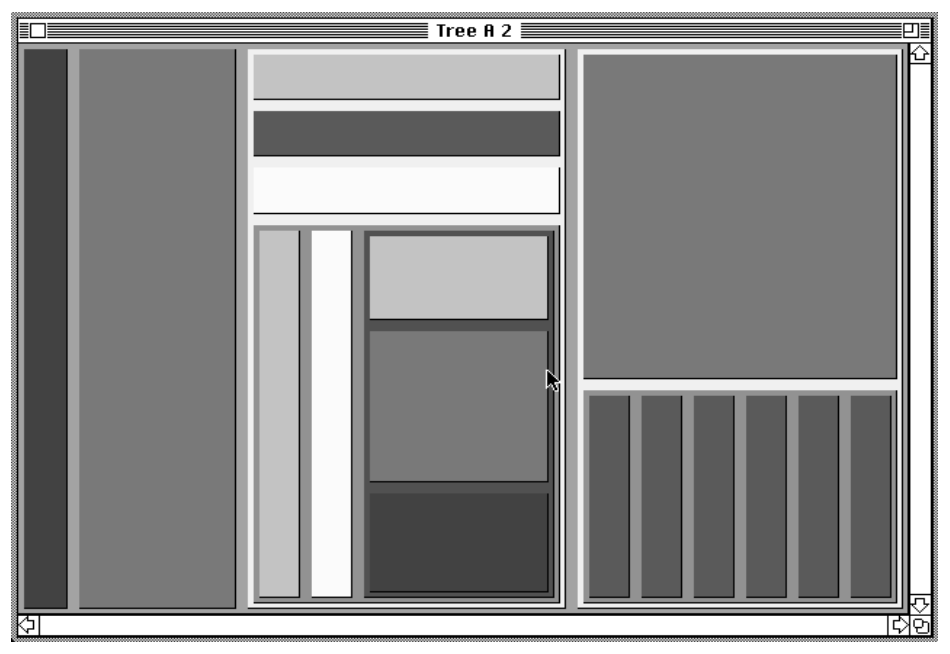
\includegraphics[width=0.5\textwidth]{images/nestedTreemapDiagramm.png}
    \caption{Beispiel für eine Treemap}
    \label{fig:nestedTreemap}
\end{figure}

Trotz der weiten Verbreitung des Ansatzes weisen Shneiderman und Johnson auf ein zentrales Problem nicht explizit hin: Der notwendige Abstand zwischen Rechtecken wird realisiert, indem von jedem Rechteck an allen vier Seiten ein Rand abgezogen wird. Dadurch ist die resultierende Fläche oftmals nicht mehr proportional zu den zugehörigen Werten. Insbesondere sehr kleine oder langgestreckte Rechtecken können im Extremfall sogar komplett verschwinden. Dies verletzt die dritte Eigenschaft (strikte Proportionalität). In praktischen Anwendungsfällen, zum Beispiel wenn die Rechtecksfläche eine Kennzahl wie \enquote{Lines of Code} darstellen soll, können kleine Dateien oder Knoten durch die Ränder also komplett verloren gehen. Problematisch ist dies insbesondere, wenn eine weitere Dimension (wie beispielsweise die Testabdeckung) diese Elemente eigentlich hervorheben sollte, sie aber infolge der Skalierung durch Randabzug nicht mehr sichtbar sind.

Ein weiteres ästhetisches Manko liegt darin, dass die rekursive Unterteilung längliche oder stark verzerrte Rechtecksformen erzeugen kann. Dies widerspricht ebenfalls dem Anspruch übersichtlicher und ansprechender Visualisierung. Verschiedene Verbesserungsansätze wie etwa \textit{Squarified Treemaps} begegnen diesem Problem und werden im Folgenden diskutiert (siehe Abschnitt \ref{sec:Squarify}).

\smallskip

%was meint häufig, hier noch so eine Quelle einfügen
In der Literatur besteht häufig Unklarheit über die Definition von 3D-Treemaps. Streng genommen bedeutet 3D-Treemap die rekursive Unterteilung eines Würfels (oder Quaders) in kleinere Volumina, wobei zum Wertvergleich das Volumen und nicht mehr die Fläche herangezogen wird. Gegenstand der vorliegenden Arbeit sind jedoch sogenannte \textit{2.5D-Treemaps}, bei denen ein klassisches 2D-Treemap-Layout um eine zusätzliche dritte Dimension (zum Beispiel durch Extrusion nach oben) erweitert wird. Im Kontext dieser Arbeit ist mit einer \enquote{3D-Darstellung} stets dieses 2.5D-Modell gemeint.


\subsubsection{Squarify-Algorithmus} \label{sec:Squarify}

Der Squarify-Algorithmus ist ein Verfahren zur Anordnung von Rechtecken in Treemaps, bei dem die Seitenverhältnisse der Rechtecke möglichst ausgeglichen gestaltet werden sollen. Ziel ist es, annähernd quadratische Rechtecke zu erzeugen, um die Nachteile herkömmlicher Treemap-Layouts zu überwinden, bei denen oft sehr schmale und langgezogene Rechtecke entstehen. Bruls et al. betonen dazu: 
\enquote{another problem of standard treemaps [is] the emergence of thin, elongated rectangles}\cite[1]{bruls2000squarified}. Rechtecke mit möglichst ähnlichen Seitenlängen sind einerseits leichter wahrzunehmen, zu vergleichen sowie in ihrer Größe intuitiv abschätzbar.

Der Squarify-Algorithmus arbeitet rekursiv, indem er die zu verteilende Fläche schrittweise in Rechtecke aufteilt. Dabei wird stets angestrebt, das Verhältnis von Breite zu Länge der Rechtecke so nah wie möglich an einen Zielwert (idealerweise $1$) zu bringen. Wie viele andere Treemap-Algorithmen erfolgt die Aufteilung vom Wurzelknoten her, indem die Fläche sukzessive in kleinere Teilflächen untergliedert wird, bis auf Blattknotenebene.

Im Folgenden wird der Algorithmus anhand eines Beispiels aus dem Originalartikel von Bruls et al. \cite[5]{bruls2000squarified} erläutert, wobei die Erklärung näher an einer praktischen Implementierung aus der d3-Bibliothek \cite{d3_treemap_code} ausgerichtet ist.

Der Algorithmus füllt die zur Verfügung stehende Fläche stets in Reihen auf, wobei in jeder Reihe möglichst quadratische Rechtecke entstehen sollen. Das Einfügen erfolgt dabei iterativ: Das erste Rechteck wird eingefügt, dann das aktuelle Seitenverhältnis des Rechtecks berechnet. Dann wird das nächste Rechteck eingefügt. Wenn durch das Einfügen das Seitenverhältnis eines Rechtecks der Reihe schlechter wird, wird eine neue Reihe eröffnet.

In dieser Arbeit wird (abweichend von einigen Publikationen) die X-Koordinate als Breite und die Y-Koordinate als Länge bezeichnet, um Verwechslungen mit der Z-Komponente (Höhe im dreidimensionalen Raum) zu vermeiden.

\smallskip

Im Folgenden wird der Algorithmus zur Anordnung von Rechtecken anhand eines konkreten Beispiels erläutert. Es sollen Rechtecke mit den Größen $6$, $6$, $4$, $3$, $2$, $2$, $1$ in ein übergeordnetes Rechteck mit den Abmessungen $6 \times 4$ einsortiert werden. 

Da das Rechteck, in welches eingefügt wird, breiter als hoch ist (Breite 6, Höhe 4), werden die Rechtecke einer vertikalen Reihe platziert. Diese vertikale Reihe, hat immer die Höhe 4 und kann nach rechts in der Breite variieren (siehe das linke große Rechteck in Abbildung \ref{fig:squarify_example_1}). Diese Reihe wird solange ergänzt, bis das schlechteste Seitenverhältnis (also das ungünstigste der enthaltenen Rechtecke) schlechter ist, als das schlechteste Seitenverhältnis im zuvorigen Schritt.

\begin{figure}
    \centering
    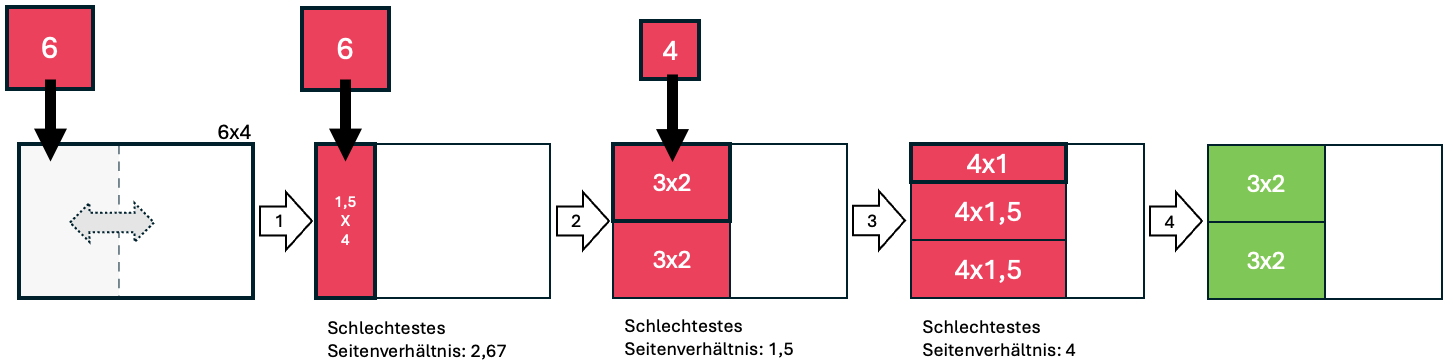
\includegraphics[width=1\textwidth]{images/squarify_example_1.png}
    \caption{Beispiel für die erste Reihe des Squarify-Algorithmus. Die Reihe ist im linken großen Rechteck in hellgrau dargestellt, die kann nach rechts in der Breite variieren. Rot sind die Rechtecke, die in ihrer Breite und Höhe noch nicht festgelegt sind. Grün sind die Rechtecke, bei denen die Breite und Höhe neu festgelegt wurde.}
    \label{fig:squarify_example_1}
\end{figure}

Zunächst wird in Schritt 1 das erste Rechteck mit einer Fläche von 6 Einheiten in die noch leere Reihe eingefügt. Das Seitenverhältnis dieses Rechtecks beträgt $1,5 \times 4$ (1,5 Einheiten breit und 4 Einheiten lang). Das schlechteste Seitenverhältnis aller Rechtecke in der aktuellen Reihe ist trivialierweise das des einzigen Rechtecks aktuell, also $4 : 1,5 \approx 2,67$ (wir teilen per Definition immer den größeren Wert durch den kleineren, dadurch ist 1 der optimale Wert, an den man sich von oben annähert, dadurch werden die vergleiche einfacher).
In Schritt zwei wird das nächste Rechteck mit einer Fläche von 6 Einheiten in die Reihe \textit{von oben} über das erste REchteck eingefügt. Dadurch wird die Reige und auch das erste Rechteck breiter. In diesem Fall haben beide Rechtecke das gleiche Seitenverhältnis von $3 \times 2$ (3 Einheiten breit und 2 Einheiten lang). Das schlechteste Seitenverhältnis in der Reihe ist nun als $3 : 2 = 1,5$ zu berechnen. Das neue schlechteste Seitenverhältnis ist also besser als das vorherige, sodass die Reihe weiter gefüllt werden kann.
Im nächsten Schritt soll ein Rechteck der Fläche 4 Einheiten eingefügt werden. Das hinzufügen dieses Rechtecks macht die Reihe erneut breiter. Es entsteht ein neues Schlechtestes Seitenverhältnis von $4 : 1 = 4$. Da das Verhältnis nun schlechter ist als das vorherige, wird die Reihe, so wie sie zuvor war, als abgeschlossen betrachtet. Das zuletzt eingefügte Rechteck (mit Fläche 4) wird daher nicht mehr in dieser Reihe, sondern in einer neuen Reihe einsortiert (siehe Schritt 4). 

\begin{figure}
    \centering
    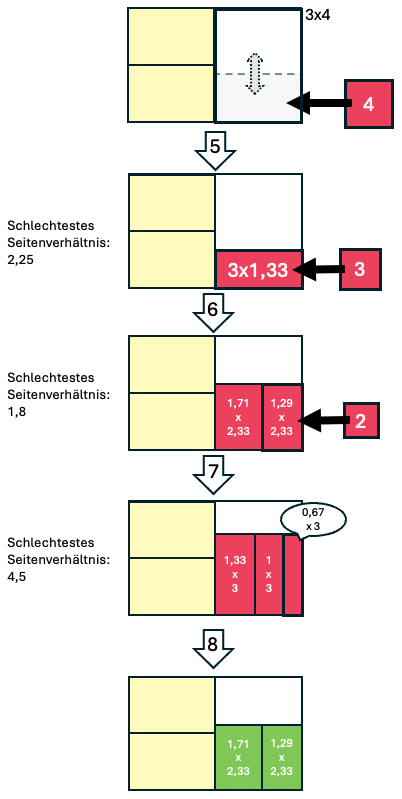
\includegraphics[width=0.7\textwidth]{images/squarify_example_2.png}
    \caption{Beispiel für die zweite Reihe des Squarify-Algorithmus. Die Reihe ist im linken großen Rechteck in hellgrau dargestellt, die kann nach rechts in der Breite variieren. Rot sind die Rechtecke, die in ihrer Breite und Höhe noch nicht festgelegt sind. Gelb sind die Rechtecke die teil von zuvor abgeschlossenen Reihen sind. Grün sind die Rechtecke, bei denen die Breite und Höhe neu festgelegt wurde.}
    \label{fig:squarify_example_2}
\end{figure}

Nachdem nun die erste Reihe abgeschlossen ist, wird eine neue Reihe eröffnet (siehe Abbildung \ref{fig:squarify_example_2}). Das durch die zuvor erstellte Reihe verbliebene, zu füllende Rechteck hat die Abmessungen $3 \times 4$ (3 Einheiten breit und 4 Einheiten lang). Da die Reihe länger als breit ist. Durch das Einfügen des Rechtecks entsteht ein schlechtestes Seitenverhältnis von $3 : 1,33 \approx 2,25$. Das Einfügen des nächsten Rechtecks mit der Fläche 3 Einheiten verbessert das schlechteste Seitenverhältnis auf $2,33 : 1,29 \approx 1,8$ und ist damit besser als das vorherige. Das Einfügen des nächsten Rechtecks mit der Fläche 2 verschlechtert das schlechteste Seitenverhältnis auf $3 : 0,67 \approx 4,5$, sodass die Reihe abgeschlossen wird (Schritt 8).

Dieser Prozess wird so lange fortgesetzt, bis alle Rechtecke in Reihen einsortiert sind (siehe Abbildung \ref{fig:squarify_examples}).

\begin{figure}
    \centering
    \begin{subfigure}{1\textwidth}
        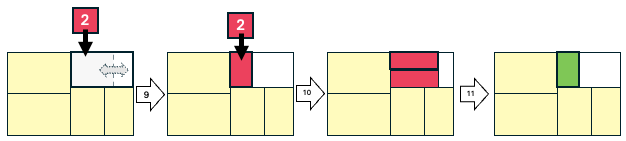
\includegraphics[width=\linewidth]{images/squarify_example_3.png}
        \caption{Reihe 3}
    \end{subfigure}
    \hfill
    \begin{subfigure}{1\textwidth}
        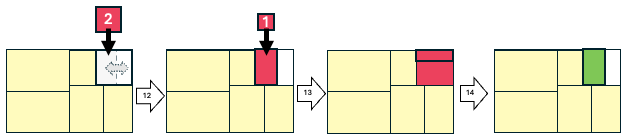
\includegraphics[width=\linewidth]{images/squarify_example_4.png}
        \caption{Reihe 4}
    \end{subfigure}
    \hfill
    \begin{subfigure}{0.4\textwidth}
        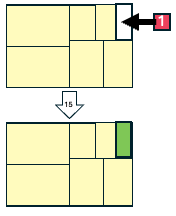
\includegraphics[width=0.7\linewidth]{images/squarify_example_5.png}
        \caption{Reihe 5}
    \end{subfigure}
    \caption{Beispiel für die letzen Reihen des Squarify-Algorithmus. Die Reihen sind im linken großen Rechteck in hellgrau dargestellt, die kann nach rechts in der Breite variieren. Rot sind die Rechtecke, die in ihrer Breite und Höhe noch nicht festgelegt sind. Gelb sind die Rechtecke die teil von zuvor abgeschlossenen Reihen sind. Grün sind die Rechtecke, bei denen die Breite und Höhe neu festgelegt wurde.}
    \label{fig:squarify_examples}
\end{figure}

\smallskip

Der Schritt, das jeweils schlechteste Seitenverhältnis in einer Reihe zu bestimmen, lässt sich rechnerisch effizient gestalten. Für ein Rechteck mit Fläche $w_i$ in einer Reihe mit konstanter Länge $l$ und Breite $w$ sowie Gesamtfläche $sV$ innerhalb der Reihe kann das maximale Seitenverhältnis durch folgende Umformungen vereinfacht berechnet werden:

\begin{align}
    \frac{w_i}{l_i} 
    &= \frac{w_i \cdot l_i \cdot w^2}{l_i \cdot l_i \cdot w^2} \\
    &= \frac{w_i \cdot l_i \cdot w^2}{l_i^2 \cdot \left(\sum_{j=0}^{n} w_j\right)^2} \\
    &= \frac{w_i \cdot l_i \cdot w^2}{\left(l_i \cdot \sum_{j=0}^{n} w_j\right)^2} \\
    &= \frac{w_i \cdot l_i \cdot w^2}{\left(\sum_{j=0}^{n} l_i \cdot w_j\right)^2} \\
    &= \frac{w_i \cdot l_i \cdot w^2}{\left(\sum_{j=0}^{n} l_j \cdot w_j\right)^2}
    \quad\text{da } \forall i, j \in \{0, \dots, n\}, l_i = l_j \\
    &= \frac{V_i \cdot w^2}{sV^2}
\end{align}

Ebenso gilt analog $ \frac{l_i}{w_i} = \frac{sV^2}{V_i \cdot w^2} $. Es genügt daher, für das jeweils größte und kleinste Rechteck in der Reihe den Wert zu berechnen und daraus das schlechteste Seitenverhältnis zu nehmen.

Während der Füllung einer Reihe bleibt $w$ konstant und muss daher nur einmal berechnet werden; $sV$ wird bei jedem neuen Rechteck in der Reihe aktualisiert.

Um den Algotihmus noch besser zu verstehen, hängen wir folgend den code an, so wie wir in in dieser Arbeit als Grundlage für die Erweiterungen verwendet haben. Der Code ist in TypeScript geschrieben. Als Vorlage für diese Implementierung diente die JavaScript-Bibliothek d3.js \cite{d3_treemap_code}.

\begin{lstlisting}[language=typescript, caption={Vereinfachte und kommentierte Grundlage für den Algorithmus der in dieser Arbeit hauptsächlich verwendet wird}, label={lst:squarify_code}]
function squarifyNode(parent: SquarifyNode) {
    // nodes sind die einzusortierenden Knoten
    const nodes: SquarifyNode[] = parent.children
    let row: SquarifyRow,
        x0 = parent.x0,
        y0 = parent.y0,
        i = 0,
        j = 0,
        numberOfChildren = nodes.length,
        width: number,
        length: number,
        value = parent.value,
        sumValue: number,
        minValue: number,
        maxValue: number,
        newRatio: number,
        minRatio: number,
        alpha: number,
        beta: number

    // i ist der Index des aktuellen Knotens, der einsortiert wird
    while (i < numberOfChildren) {
        // Ein Schleifendurchlauf entspricht einer Reihe von Knoten
        // Breite und Länge des noch zu belegenden Bereichs müssen nach jeder Reihe neu berechnet werden
        width = parent.x1 - x0
        length = parent.y1 - y0

        // Suche den nächsten Knoten mit Wert und aktualisiere den sumValue
        do {
            sumValue = nodes[j++].value
        } while (!sumValue && j < numberOfChildren)

        // minValue ist der kleinste Wert in der Reihe
        // maxValue ist der größte Wert in der Reihe
        // sumValue ist die Summe der Werte der Knoten in der aktuellen Reihe
        minValue = maxValue = sumValue
        // alpha ist der feste Faktor für die Berechnung des Seitenverhältnisses
        alpha = Math.max(length / width, width / length) / (value * aimedRatio)
        // beta ist der variable Faktor für die Berechnung des Seitenverhältnisses
        beta = sumValue * sumValue * alpha
        // minRatio speichert das aktuelle schlechteste Seitenverhältnis in der Reihe
        minRatio = Math.max(maxValue / beta, beta / minValue)

        // Füge weitere Knoten hinzu, solange sich das Seitenverhältnis nicht verschlechtert
        for (; j < numberOfChildren; ++j) {
            const nodeValue = nodes[j].value
            sumValue += nodeValue
            if (nodeValue < minValue) {
                minValue = nodeValue
            }
            if (nodeValue > maxValue) {
                maxValue = nodeValue
            }
            beta = sumValue * sumValue * alpha
            // Berechne das neue schlechteste Seitenverhältnis nach dem Hinzufügen des Knotens
            newRatio = Math.max(maxValue / beta, beta / minValue)

            if (newRatio > minRatio) {
                // Wenn das Seitenverhältnis schlechter wird, entferne den letzten Knoten und beende die Schleife
                sumValue -= nodeValue
                break
            }
            minRatio = newRatio
        }

        // Fülle die Reihe mit den ausgewählten Knoten und berechne deren Position und Größe
        row = { name: parent.name, value: sumValue, dice: width < length, children: nodes.slice(i, j) }
        if (row.dice) {
            treemapDice(row, x0, y0, parent.x1, value ? (y0 += (length * sumValue) / value) : y0)
        } else {
            treemapSlice(row, x0, y0, value ? (x0 += (width * sumValue) / value) : x0, parent.y1)
        }

        // Der noch zu belegende Bereich wird um die Größe der aktuellen Reihe verkleinert
        value -= sumValue
        i = j
    }
}
\end{lstlisting}

\smallskip

Obwohl sich das ursprüngliche Paper von Bruls et al. \cite{bruls2000squarified} vor allem auf das Seitenverhältnis $1$ als Idealwert konzentriert, erlauben viele Implementierungen, wie auch die implementierungen von d3.js \cite{d3_treemap_code} auch die Annäherung an andere Zielwerte, beispielsweise an den Goldenen Schnitt \cite{goldenRatio}. 
In Abbildung \ref{fig:squarifyRatio1} ist ein Beispiel für ein Layout zu sehen, dass durch den Squarify-Algorithmus generiert wurde, wobei die Rechtecke möglichst quadratisch werden sollen, so wie beim Original-Algorithmus von Bruls et al. \cite{bruls2000squarified}. In Abbildung \ref{fig:squarifyRatio5} sind die selben Werte zu sehen. Day layout wurde auch durch den Squarify-Algorithmus generiert, jedoch mit dem Ziel, dass die Rechtecke ein Seitenverhältnis von 5 anstreben. Es ist ein deutlicher Unterschied in den Darstellungen zu erkennen: Die Rechtecke sind deutlich langgestreckter, als im ersten Beispiel.

\begin{figure}[h]
    \centering
    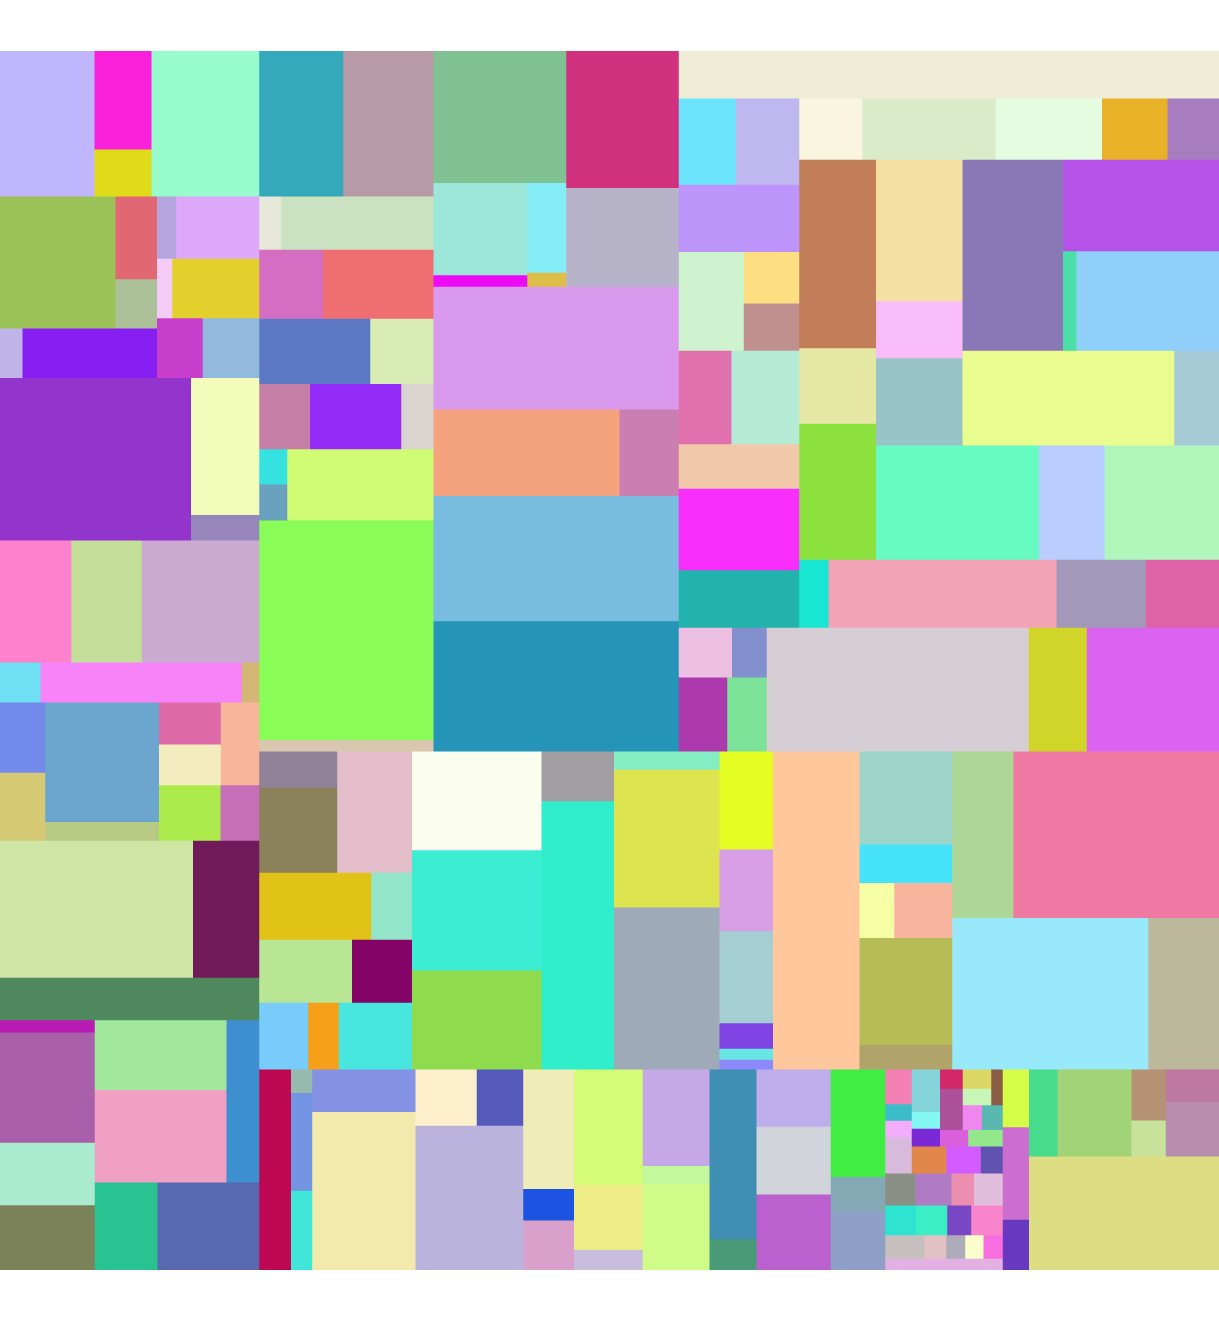
\includegraphics[width=0.5\textwidth]{images/oneSquarify.png}
    \caption{Beispiel für ein Squarify-Layout mit Annäherung an quadratische Rechtecke (durchschnittliches Seitenverhältnis 1,42)}
    \label{fig:squarifyRatio1}
\end{figure}

\begin{figure}[h]
    \centering
    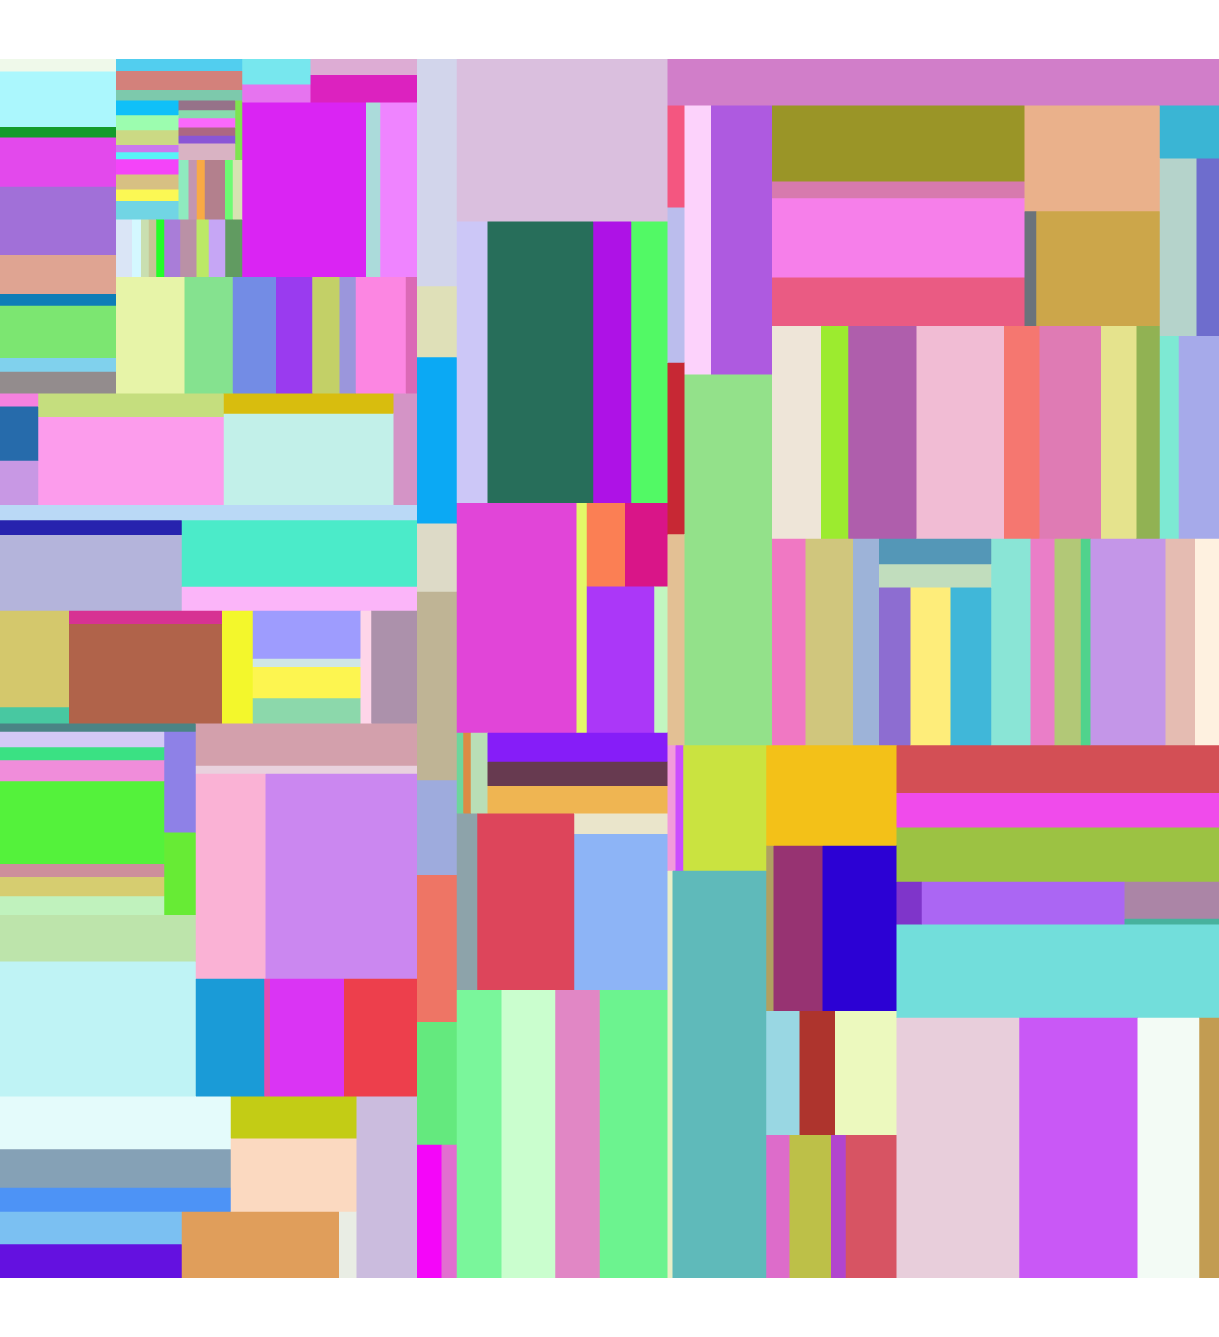
\includegraphics[width=0.5\textwidth]{images/fiveSquarify.png}
    \caption{Beispiel für ein Squarify-Layout mit Annäherung an den Wert 5 (durchschnittliches Seitenverhältnis 2,79)}
    \label{fig:squarifyRatio5}
\end{figure}